\documentclass{beamer}
\usepackage[brazilian]{babel}
\usepackage[utf8]{inputenc}
\usepackage{hyperref}
\usepackage{calc}
\usepackage[absolute,overlay]{textpos}
\usepackage{tikz}
\usetikzlibrary{trees}
\usetikzlibrary{decorations.pathmorphing}
\usetikzlibrary{decorations.markings}
%\usepackage[usestackEOL]{stackengine}
%\def\title#1{\centerline{\LARGE\bf\Longstack{#1}}\vskip .5em}
\mode<presentation>{\usetheme{tud}}

\title[Quenching with Hydro]{Quenching with Hydro}
\subtitle{A study of Jet Quenching properties using $\rm JEWEL$ framework coupled with $\rm v-USPhydro$ for hydrodynamic simulation along with $\rm T_{R}ENTo$ initial conditions}
\institute[HEPIC-Instituto de Física]{HEPIC - Instituto de Física da USP}
%\author{Fabio Canedo \and Marcelo G Munhoz \and J Noronha-Hostler \and J Noronha \and Caio Prado}
\date{\today}



% Insert frame before each subsection (requires 2 latex runs)
\AtBeginSubsection[] {
	\begin{frame}<beamer>\frametitle{\titleSubsec}
		\tableofcontents[currentsection,currentsubsection]  % Generation of the Table of Contents
	\end{frame}
}
% Define the title of each inserted pre-subsection frame
\newcommand*\titleSubsec{Content}
% Define the title of the "Table of Contents" frame
\newcommand*\titleTOC{Content}

% define a symbol which can be removed if you don't need it
\newcommand{\field}[1]{\mathbb{#1}}
\newcommand{\Zset}{\field{Z}}

\setbeamerfont{footnote}{size=\tiny}

\begin{document}

{
% remove the next line if you don't want a background image
%\usebackgroundtemplate{}%
\setbeamertemplate{footline}{\usebeamertemplate*{minimal footline}}
\frame{\titlepage}
}

{\setbeamertemplate{footline}{\usebeamertemplate*{minimal footline}}
\begin{frame}\frametitle{\titleTOC}
	\tableofcontents
\end{frame}
}

\section{Introduction}
\subsection{Jet Quenching}

\begin{frame}\frametitle{Jet Quenching}
	\begin{columns}
	\begin{column}{0.5\textwidth}
	\onslide<1->{\textbf{Motivation}}
	\onslide<2->{\\ Study Jet Quenching on a realistic enviroment.}
	\onslide<3->{Several models: {\tiny
		\begin{itemize}
		\item<4-> Ya-JEM;
		\item<5-> JEWEL;
		\item<6-> MARTINI;
		\item<7-> Q-PYTHIA;
		\end{itemize}}
	}
	\onslide<8->{Must use realistic medium evolution} \\
	\onslide<9->{Must be able to make differential predictions}
	\end{column}
	\begin{column}{0.5\textwidth}
	\only<1-8>{
	\begin{figure}
	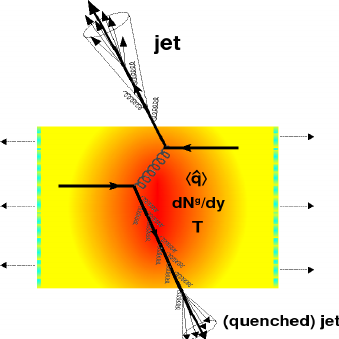
\includegraphics[width=1\textwidth]{images/quenching.png}
	\end{figure}
	}
	\only<9->{
	\tikzset{
    photon/.style={decorate, decoration={snake}, draw=red},
    electron/.style={draw=white, postaction={decorate},
        decoration={markings,mark=at position .55 with {\arrow[draw=white]{>}
        ,amplitude=0.4mm}}},
    positron/.style={draw=white, postaction={decorate},
      	decoration={markings,mark=at position .55 with {\arrow[draw=white]{<}
      	,amplitude=0.4mm}}},
    gluon/.style={decorate, draw=yellow,
        decoration={coil,amplitude=0.4mm, segment length=0.5mm}} 
	}
	\begin{tikzpicture}[
        thick,
        % Set the overall layout of the tree
        level/.style={level distance=3mm},
        level 2/.style={sibling distance=3mm},
        level 3/.style={sibling distance=3mm}
    ]
	\node[inner sep=0pt] (russell) at (0,0)
    {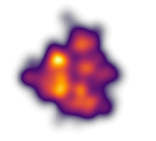
\includegraphics[width=1\textwidth]{images/trento_quenching.png}};
    \coordinate
    	child[grow=up]{    		
    		child{
    		child{edge from parent[gluon]}
    			child{
    				child{
    					child{edge from parent[electron]}
    					child{edge from parent[gluon]}
    				edge from parent[electron]
    				}
    			edge from parent[electron]
    			}
    		edge from parent[electron]
    		}
    		child{edge from parent[gluon]}
    	edge from parent[electron]
    	}
    	child[grow=down]{
    		child{
    		child{edge from parent[gluon]}
    			child{
    				child{
    					child{edge from parent[electron]}
    					child{edge from parent[gluon]}
    				edge from parent[electron]
    				}
    			edge from parent[electron]
    			}
    		edge from parent[electron]
    		}
    		child{edge from parent[gluon]}
    	edge from parent[electron]}
    ;
	\end{tikzpicture}
	}
	\end{column}
	\end{columns}
\end{frame}

\begin{frame}\frametitle{JEWEL}
	\textbf{JEWEL$^{a,b,c}$(Jet Evolution with Energy Loss)}
	\begin{columns}
	\begin{column}{0.4\textwidth}
	\begin{itemize}
	\small
	\item<2-> Runs along with PYTHIA;
	\item<3-> Based on BDMPS-Z formalism;
	\item<4-> Perturbative and minimal in assumptions;
	\item<5-> Allows differential and geometric treatment(jet shape);
	\end{itemize}
	{\tiny
	$^{a}$ Eur.Phys.J. C74 (2014) no.2,2762 [arXiv:1212.1599] \\
	$^{b}$ JHEP 1303 (2013) 080 [arXiv:0804.3568] \\
	$^{c}$ arXiv:1707.01539
	}
	
	\end{column}
	\begin{column}{0.6\textwidth}
	\begin{figure}
	\includegraphics<1->[width=0.6\textwidth]{images/feynman.png}
	\end{figure}
	\end{column}
	\end{columns}
\end{frame}

\subsection{Initial conditions}
\begin{frame}\frametitle{Default}
	Smooth Glauber\footnote{JEWEL Default}
	\begin{equation*}
	\begin{split}
	n(b,x,y) &= T_A(x-\frac{b}{2},y) \left( 1-\exp\left(- \sigma_{NN} T_B(x+\frac{b}{2},y) \right) \right) \\
	&+ T_B(x+\frac{b}{2},y) \left( 1-\exp\left(- \sigma_{NN} T_A(x-\frac{b}{2},y) \right) \right)
	\end{split}
	\end{equation*}
	\pause
	Where:
	\begin{equation*}
	T(x,y) = \int dz \rho(x,y,z)
	\end{equation*}
	And $\rho$ is the Woods-Saxon potential.
\end{frame}

\begin{frame}\frametitle{$\rm T_{R}ENTo$}
	\onslide<1->{\textbf{$\rm T_{R}ENTo$}$\,^{a}$} \\
	\begin{itemize}
	\item<2-> parametric model based on Glauber;
	\item<3-> includes fluctuations event-by-event;
	\end{itemize}
	\begin{figure}[b]
	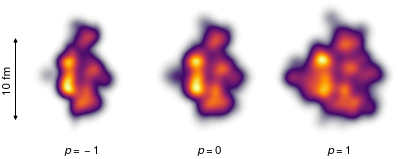
\includegraphics[width=1\textwidth]{images/trento_events_p.png}
	\end{figure}
	\onslide<1->{\tiny $\,^{a}$ arXiv:1412.4708 [nucl-th]}
\end{frame}

\begin{frame}\frametitle{MC-KLN}
	\onslide<1->{\textbf{MK-KLN}$^a$ \\
	Based on CGC with kt factorization}
	\begin{figure}[b]
	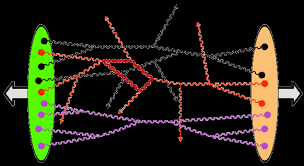
\includegraphics[height=0.3\paperheight]{images/kln.png}
	\end{figure}
	\onslide<1->{\tiny $\,^{a}$ arXiv:0707.0249 [nucl-th]}
\end{frame}

\subsection{Medium Evolution}
\begin{frame}\frametitle{Bjorken}
	A variant of the Bjorken model is used. The (proper)time dependence is given by
	\begin{equation*}
	\epsilon (x,y,b,\tau)=\epsilon(x,y,b,\tau_i) \left(\frac{\tau}{\tau_i} \right)^{-4/3}
	\end{equation*}
	and
	\begin{equation*}
	T (x,y,b,\tau)\propto\epsilon^{1/4}(x,y,b,\tau_i) \left(\frac{\tau}{\tau_i} \right)^{-1/3}
	\end{equation*}
\end{frame}

\begin{frame}\frametitle{v-USPhydro}
\begin{columns}
\begin{column}{0.5\textwidth}
   \textbf{v-USPhydro}$\,^{a}$ \\ 
   \begin{itemize}
   \item<2-> smoothed particle hydrodynamics(Lagrangian method);
   \item<3-> 2+1 dimensions;
   \item<4-> both shear viscosity($\frac{\eta}{s}=0.1$);
   \end{itemize}
   \onslide<1->{\tiny $\,^{a}$ Phys. Rev. C 90, 034907 (2014) \\ $\, \, \,$ Phys. Rev. C 88, 044916 (2013)}
\end{column}
\begin{column}{0.5\textwidth}
    \begin{figure}
	\includegraphics<1->[width=1\textwidth]{images/vusp.png}
	\end{figure}
\end{column}
\end{columns}
\end{frame}

\section{Methods}
\subsection{Jet Algorithm}
\begin{frame}\frametitle{Jet Algorithm}
	\begin{columns}
	\begin{column}{0.3\textwidth}
	Jets are defined through an algorithm that must satisfy certain conditions.
	\begin{itemize}
	\item<2-> collinear safe;
	\item<3-> infrared safe;
	\end{itemize}
	\end{column}
	\begin{column}{0.7\textwidth}
	\only<2>{
	\begin{figure}
	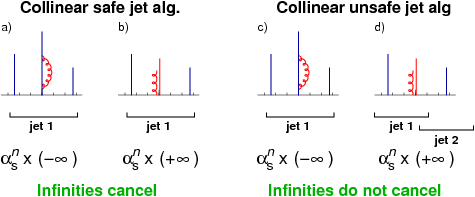
\includegraphics[width=1\textwidth]{images/collinear_safe.png}
	\end{figure}
	}
	\only<3>{
	\begin{figure}
	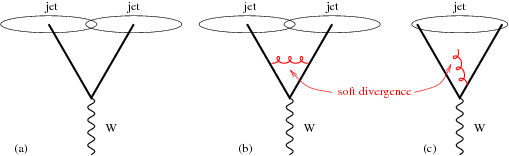
\includegraphics[width=1\textwidth]{images/infrared_safe.png}
	\end{figure}
	}
	\only<4->{
	\textbf{Anti-kt}
	\begin{figure}
	\includegraphics<4->[width=0.7\textwidth]{images/anti_kt.png}
	\end{figure}
	}
	\end{column}
	\end{columns}	
\end{frame}

\begin{frame}\frametitle{Anti-kt}
	Based on a two particle distance;
	\begin{equation*}
		d_{ij} = \min({p_{t\,i}}^{-2},{p_{t\, j}}^{-2}) \Delta \rm R_{ij}
	\end{equation*}
	\begin{equation*}
		d_{i} = {p_{t \, i}}^{-2} \Delta \rm R_{iB}
	\end{equation*}	
	Where:
	\begin{equation*}
		\Delta {\rm R} = \sqrt{ \Delta \phi^2 + \Delta \eta^2}
	\end{equation*}
\end{frame}

\subsection{Jet Observables}
\begin{frame}\frametitle{Jet Observables}
	\begin{columns}
	\begin{column}{0.5\textwidth}
	The observables chosen were the following:
	\begin{itemize}
		\item<2-> Mass;
		\item<3-> Girth;
		\item<4-> Dispersion;
		\item<5-> $v_2$;
	\end{itemize}
	\end{column}
	\begin{column}{0.5\textwidth}
	\only<2>{
	\begin{equation*}
		M_{jet} = {p_{jet}}^{\mu} {p_{jet}}_{\mu} 
	\end{equation*}
	}
	\only<3>{
	\begin{equation*}
		g = \frac{\sum_{i} p_i^{T} \Delta R_i}{p_{J}^{T}}
	\end{equation*}
	}
	\only<4>{
	\begin{equation*}
		p^T_{D} = \frac{\sqrt{\sum_{i} {p_i^{T}}^2}}{p_{J}^{T}}
	\end{equation*}
	}
	\only<5>{
	\begin{figure}
	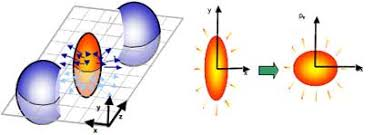
\includegraphics[width=1\textwidth]{images/index.jpeg}
	\end{figure}
	}
	\end{column}
	\end{columns}		
\end{frame}

\subsection{Thermal Subtraction}
\begin{frame}\frametitle{Thermal Subtraction}
	\textbf{JEWEL keeps recoil} \\
	\onslide<2->{Thermal contamination must be subtracted} \\
	\onslide<3->{4 Moment Subtraction:}
	\onslide<4->{Thermal momenta $\longrightarrow$ ghost particles}
	\onslide<5->{Particles close enough to these ghost particles are classified as thermal momenta.}
	\onslide<6->{4 thermal momenta summed up and subtracted from the observable.}
\end{frame}

\section{Results}

\subsection{Shape}
\begin{frame}\frametitle{Mass}
    \begin{columns}
    \begin{column}{0.6\textwidth}
	\begin{figure}
	\only<1>{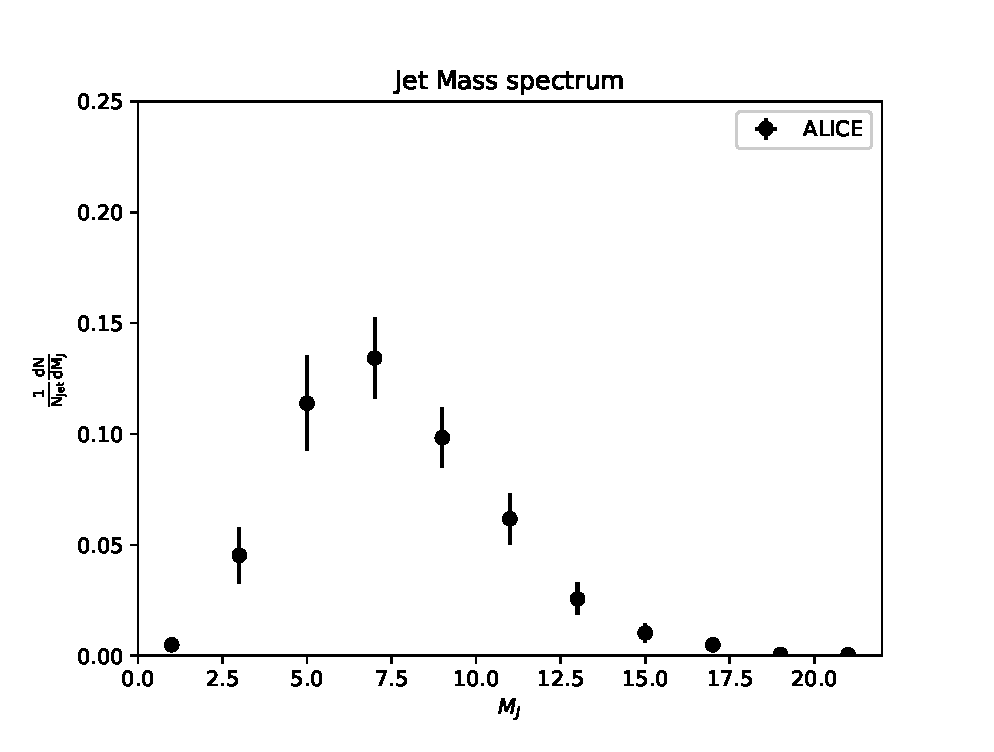
\includegraphics[width=1\textwidth]{images/Mass_1.eps}}
	\only<2>{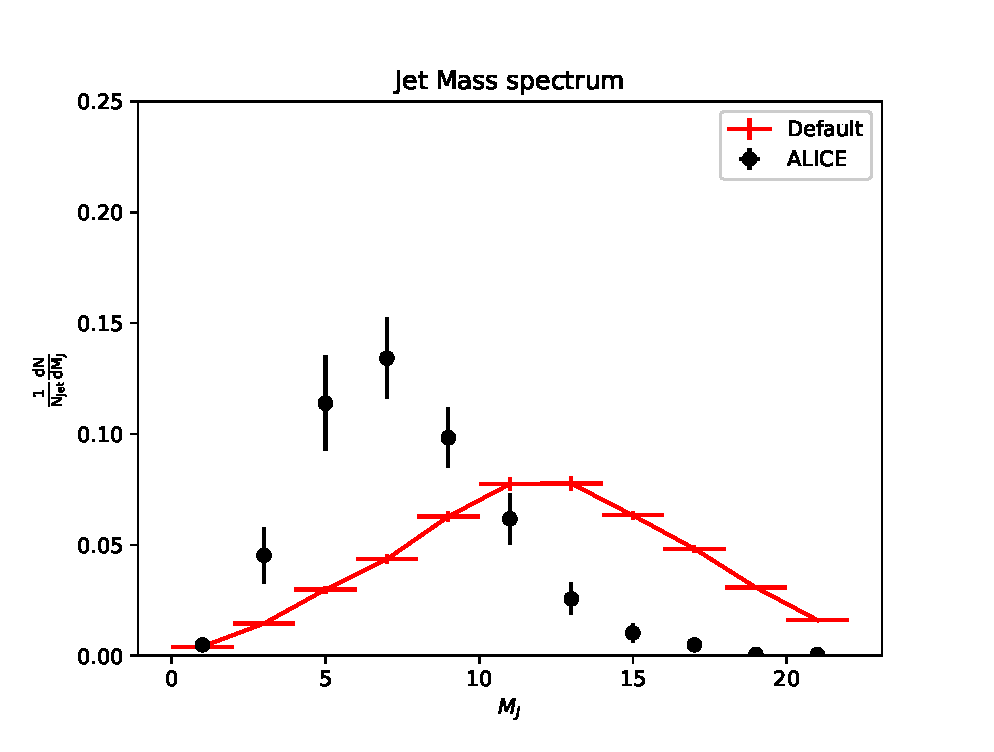
\includegraphics[width=1\textwidth]{images/Mass_2.eps}}
	\only<3>{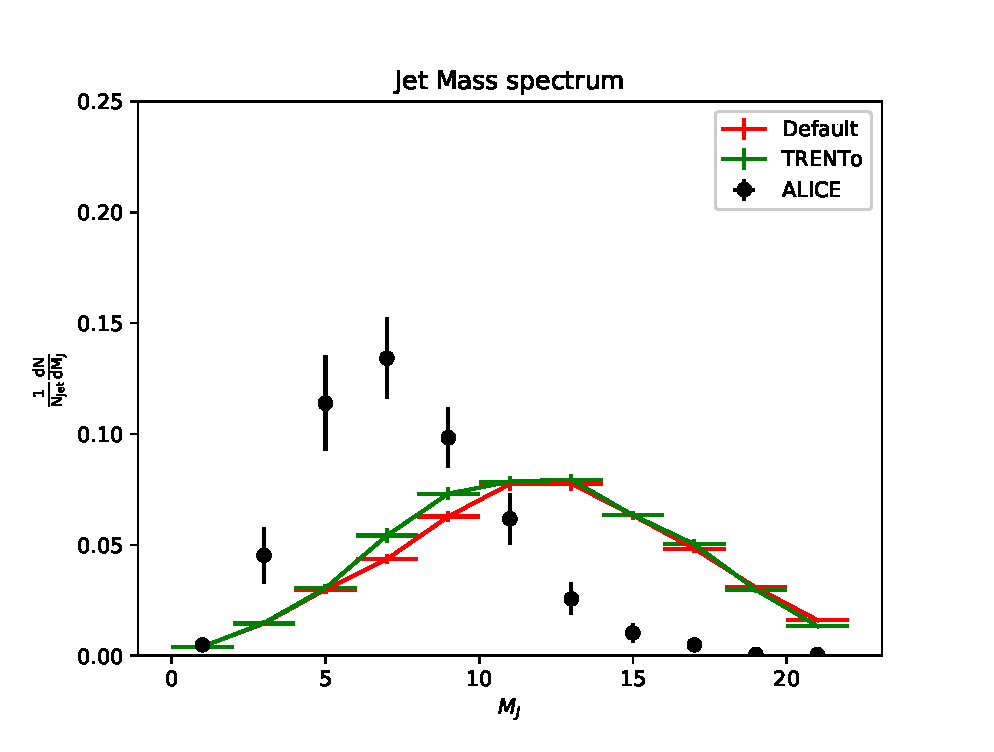
\includegraphics[width=1\textwidth]{images/Mass_3.eps}}
	\only<4>{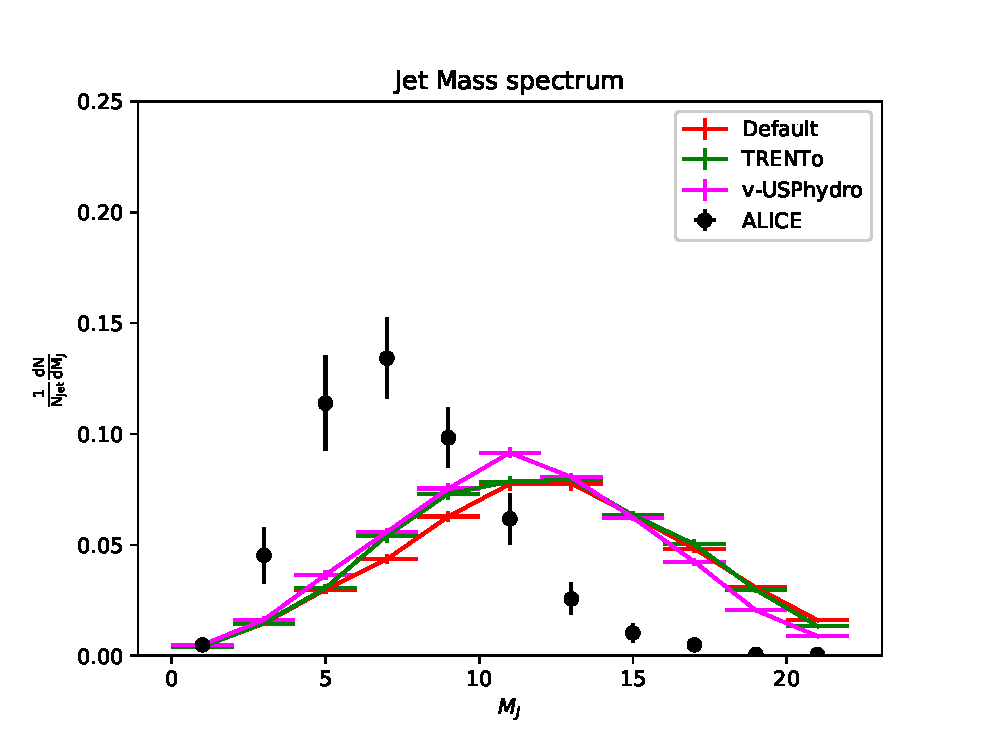
\includegraphics[width=1\textwidth]{images/Mass_4.eps}}
	\end{figure}
	\end{column}
    \begin{column}{0.4\textwidth}
	{
	anti-kt $R=0.4$ \\
	$\vert\eta\vert<0.8$ \\
	$40\,\rm{GeV/c}<p_T<60\,\rm{GeV/c}$
	}
	\end{column}
	\end{columns}
\end{frame}

\begin{frame}\frametitle{Girth}
    \begin{columns}
    \begin{column}{0.6\textwidth}
	\only<1>{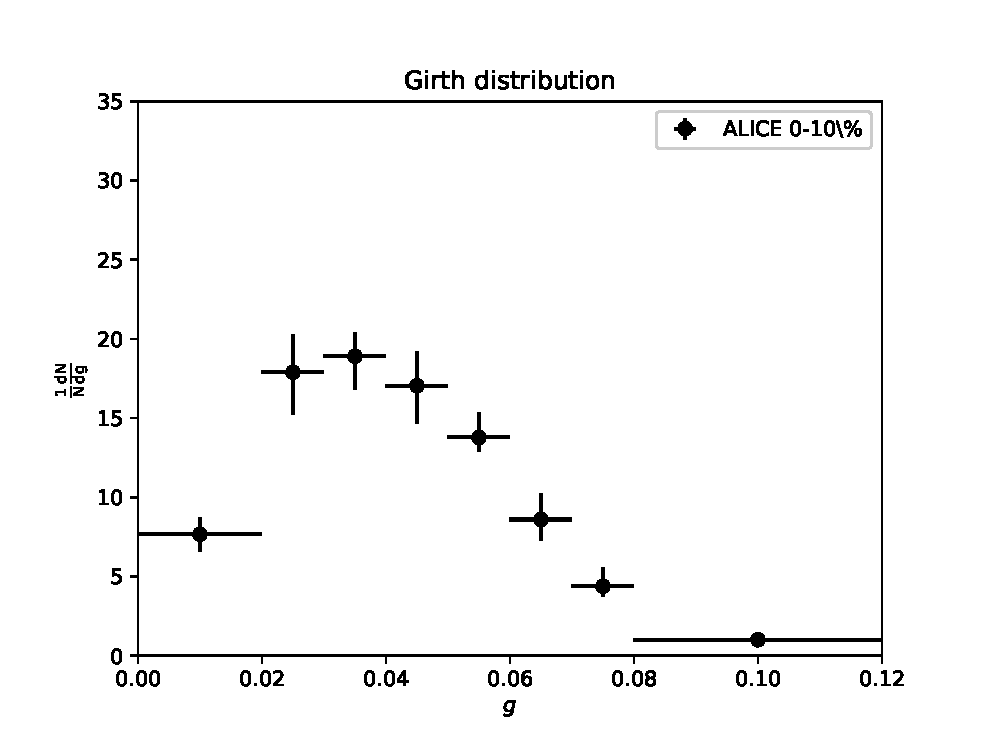
\includegraphics[width=1\textwidth]{images/My_Angularity_1.eps}}
	\only<2>{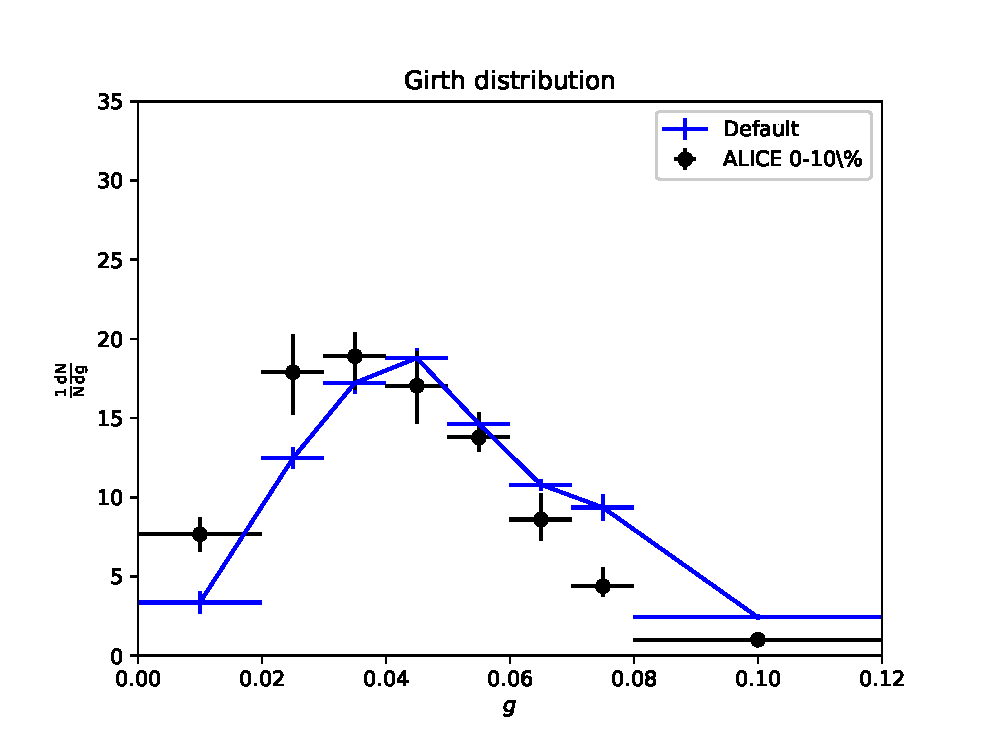
\includegraphics[width=1\textwidth]{images/My_Angularity_2.eps}}
	\only<3>{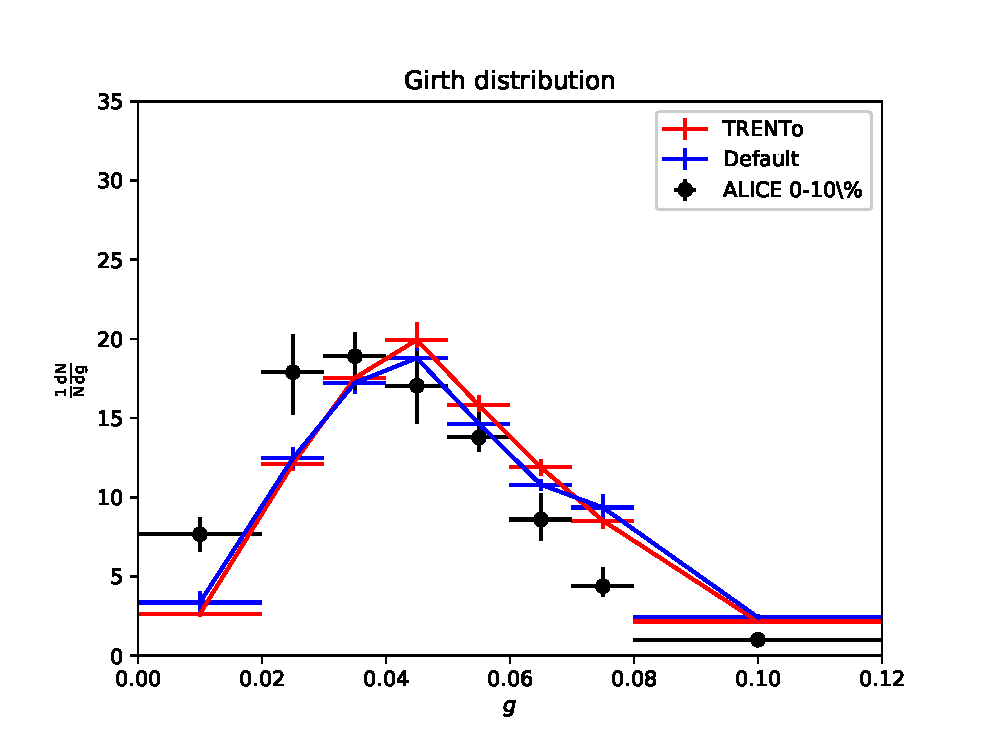
\includegraphics[width=1\textwidth]{images/My_Angularity_3.eps}}
	\only<4>{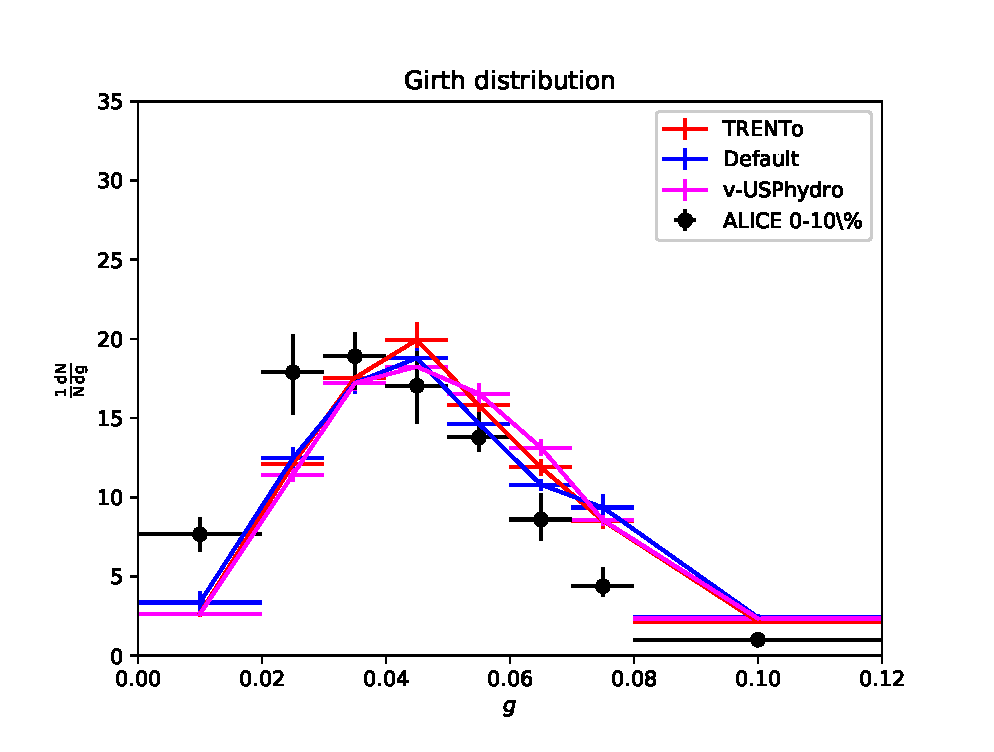
\includegraphics[width=1\textwidth]{images/My_Angularity_4.eps}}
	\end{column}
    \begin{column}{0.4\textwidth}
    {
	PbPb
	$\sqrt{\rm{s}_{\rm{NN}}} = 2.76\, \rm{TeV}$
	anti-kt $R=0.2$ \\
	$\vert\eta\vert<0.8$ \\
	$40 \, \rm{GeV/c}<p_T< 60 \, \rm{GeV/c}$
	}
	\begin{equation*}
		g = \frac{\sum_{i} p_i^{T} \Delta R_i}{p_{J}^{T}}
	\end{equation*}
	\end{column}
	\end{columns}
\end{frame}

\begin{frame}\frametitle{Dispersion}
    \begin{columns}
    \begin{column}{0.6\textwidth}
	\only<1>{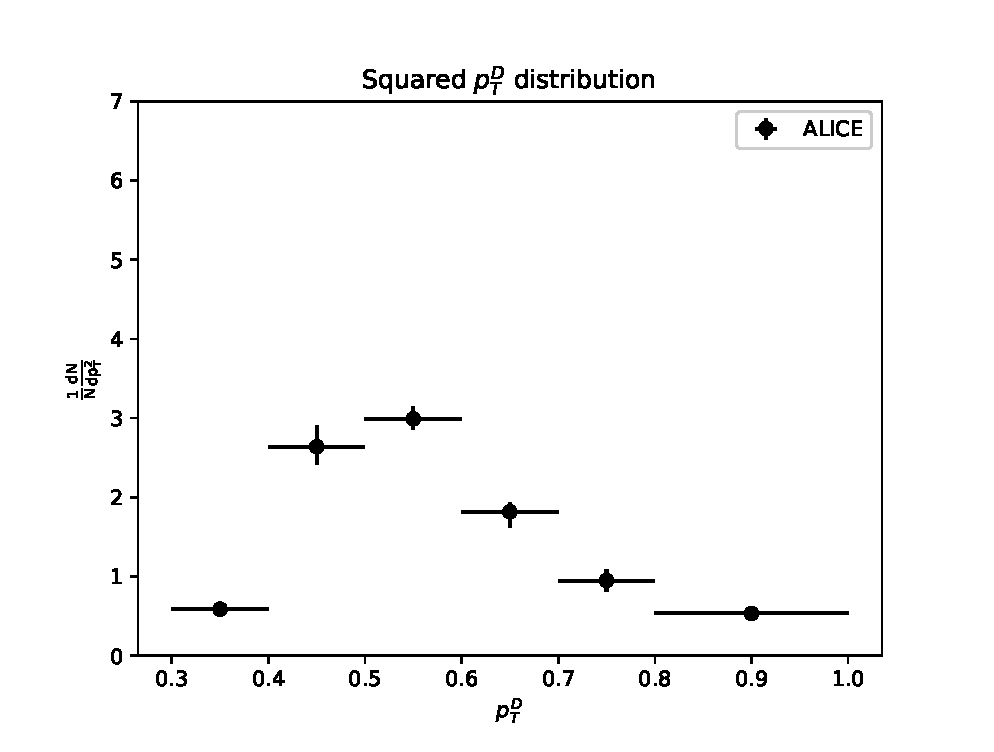
\includegraphics[width=1\textwidth]{images/Squared_1.eps}}
	\only<2>{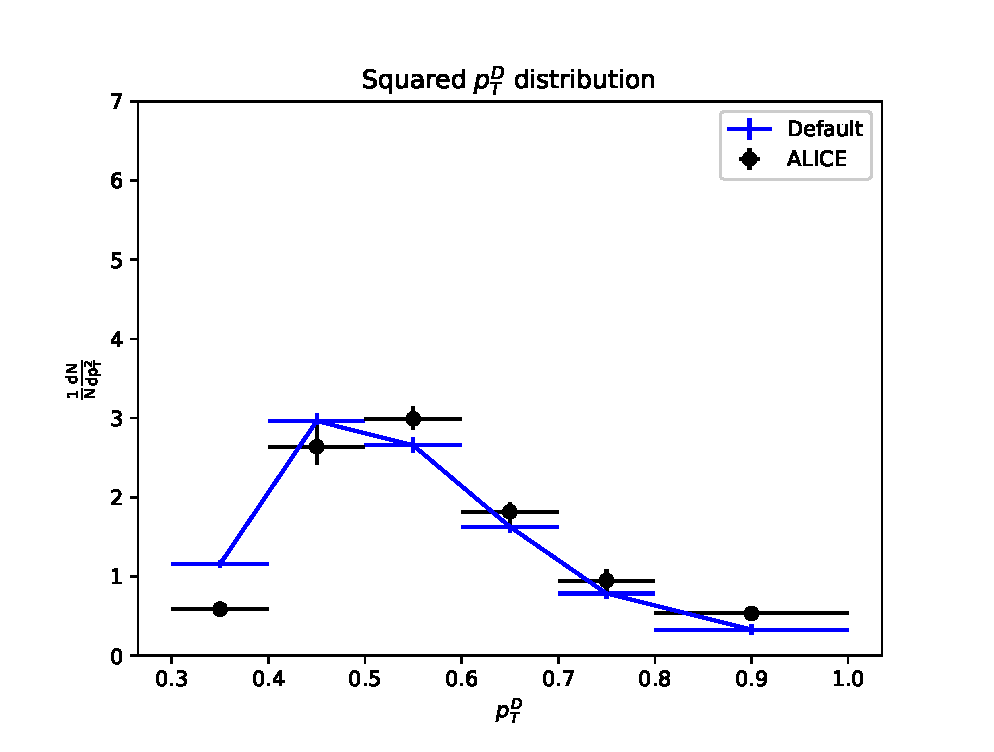
\includegraphics[width=1\textwidth]{images/Squared_2.eps}}
	\only<3>{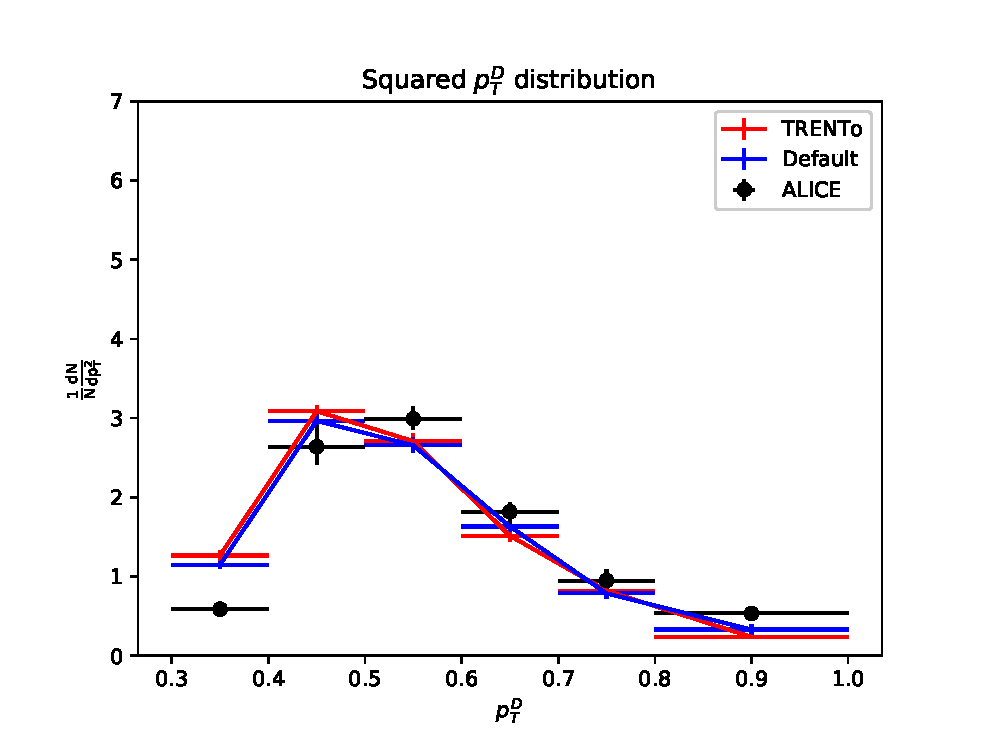
\includegraphics[width=1\textwidth]{images/Squared_3.eps}}
	\only<4>{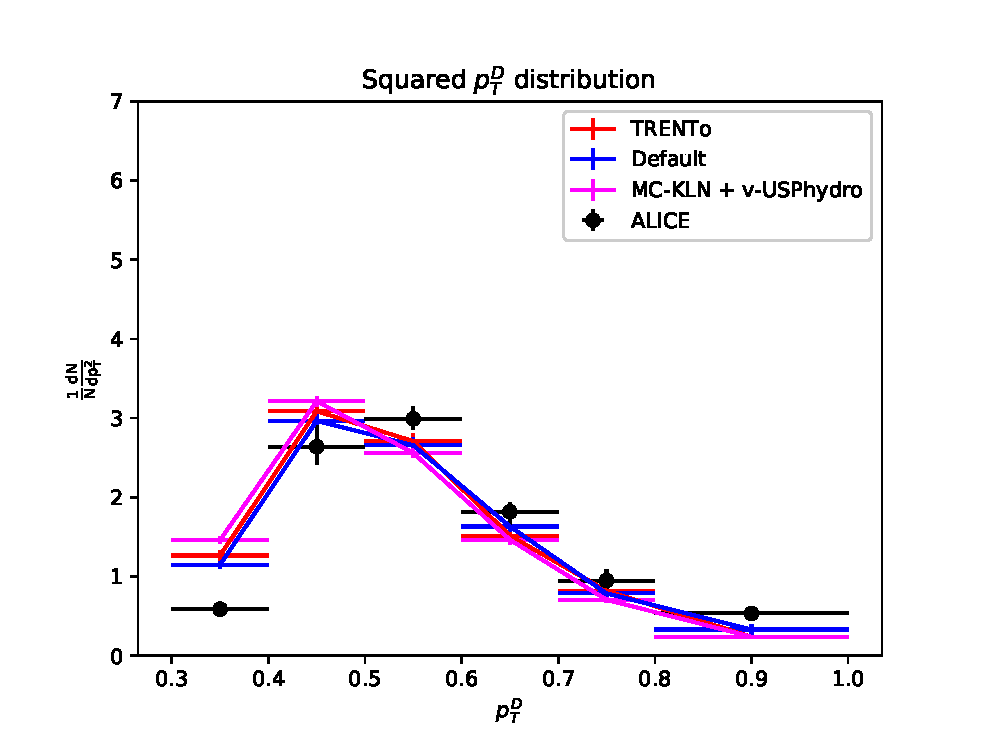
\includegraphics[width=1\textwidth]{images/Squared_4.eps}}
	\end{column}
    \begin{column}{0.4\textwidth}
	{
	PbPb 0-10\%
	$\sqrt{\rm{s}_{\rm{NN}}} = 2.76 \rm{TeV}$
	anti-kt $R=0.2$ \\
	$\vert\eta\vert<0.8$ \\
	$40 \, \rm{GeV/c} < p_T < 60 \, \rm{GeV/c}$
	}
	\begin{equation*}
		p^T_{D} = \frac{\sqrt{\sum_{i} {p_i^{T}}^2}}{p_{J}^{T}}
	\end{equation*}
	\end{column}
	\end{columns}
\end{frame}

\subsection{$v_2$}
\begin{frame}\frametitle{$v_2$}
    \begin{columns}
    \begin{column}{0.6\textwidth}
	\only<1>{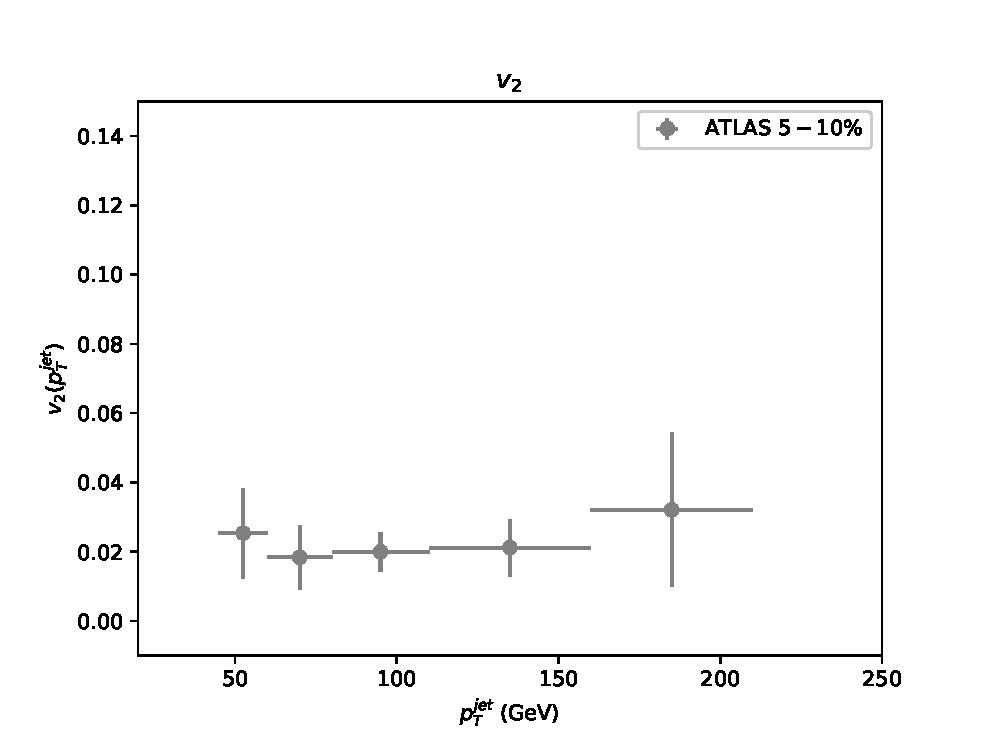
\includegraphics[width=1\textwidth]{images/v2_1.eps}}
	\only<2>{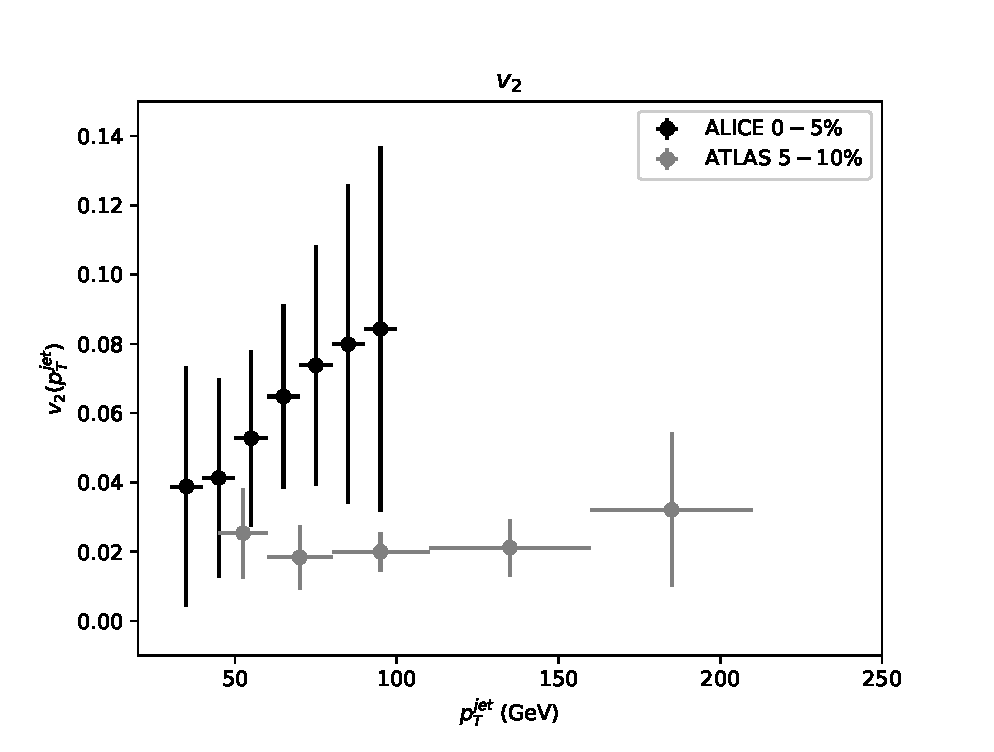
\includegraphics[width=1\textwidth]{images/v2_2.eps}}
	\only<3>{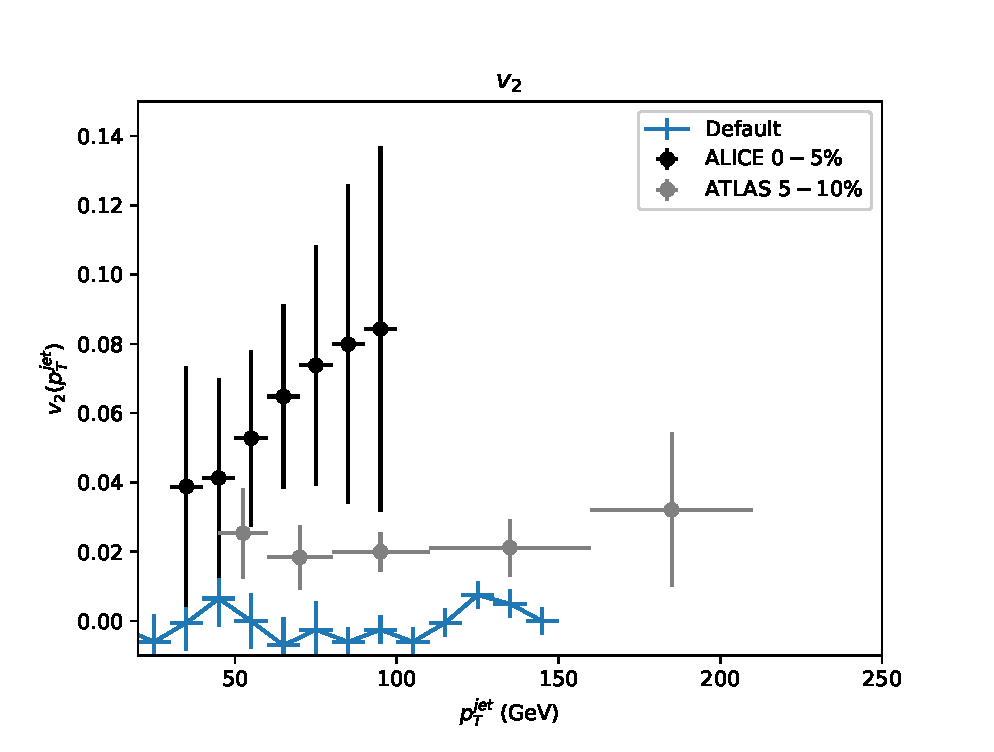
\includegraphics[width=1\textwidth]{images/v2_3.eps}}
	\only<4>{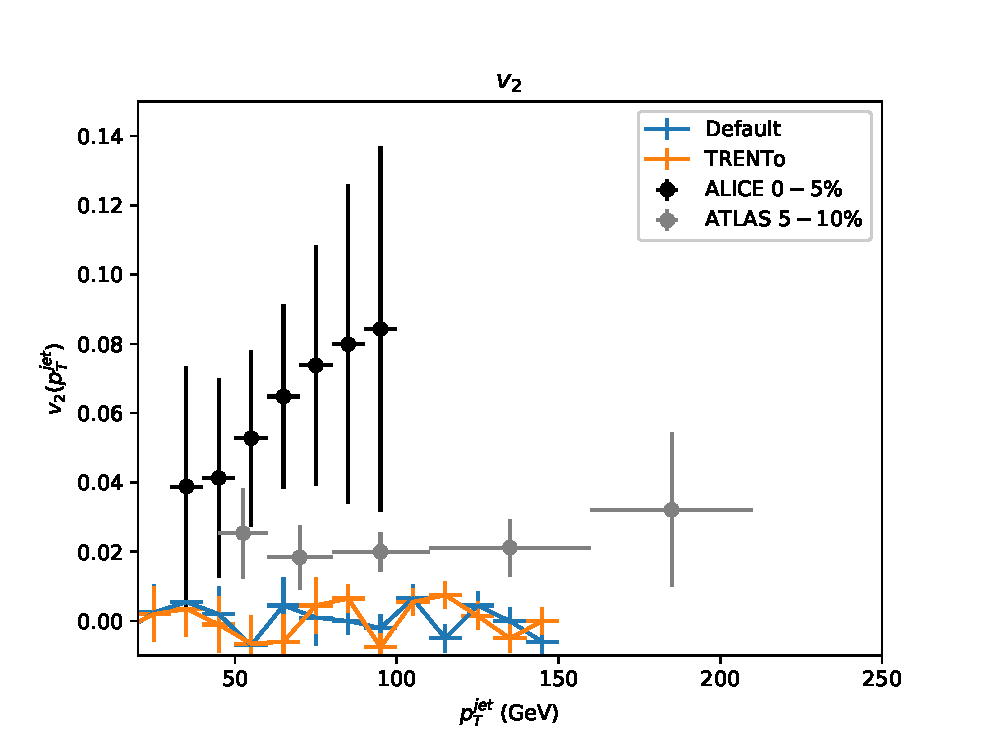
\includegraphics[width=1\textwidth]{images/v2_4.eps}}
	\only<5>{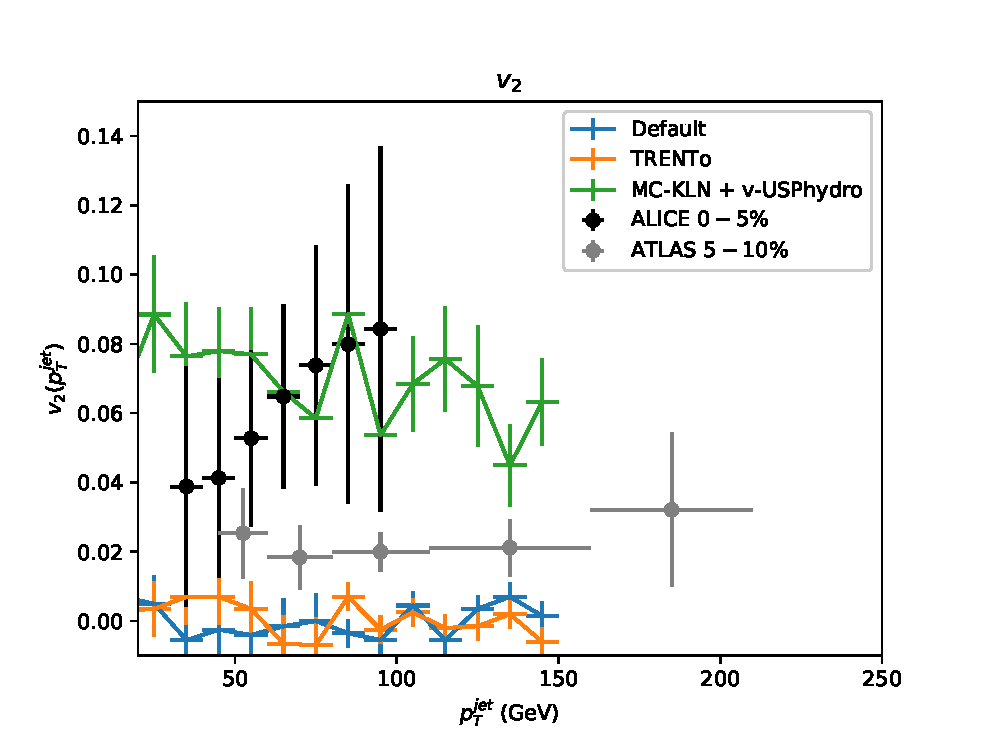
\includegraphics[width=1\textwidth]{images/v2_5.eps}}
	\end{column}
    \begin{column}{0.4\textwidth}
	PbPb
	$\sqrt{\rm{s}_{\rm{NN}}} = 2.76 \, \rm{TeV}$
	anti-kt $R=0.4$ \\
	$\vert\eta\vert<0.8$
	\end{column}
	\end{columns}
\end{frame}

\section{Conclusions and Outlook}
\begin{frame}\frametitle{Conclusions and Outlook}
\begin{itemize}
	\item<2-> The models for Jet Quenching are sensitive to more realistic hydro;
	\item<3-> Observables that look at event-by-event fluctuations might give further constraint both on hydro models and on the Jet Quenching models themselves;
	\item<4-> In the future, more systematic studies will be done;
	\item<5-> Determine which observables depend on which specific features of the hydro and initial conditions models;
\end{itemize}
\end{frame}

\begin{frame}
\large Thanks!
\end{frame}


\end{document}
